\documentclass[12pt]{article}
 
\usepackage[margin=1in]{geometry}
\usepackage{amsmath,amsthm,amssymb}
\usepackage[utf8]{inputenc}
\usepackage{graphicx}
\usepackage[T1]{fontenc}
\newcommand{\N}{\mathbb{N}}
\newcommand{\R}{\mathbb{R}}
\newcommand{\Z}{\mathbb{Z}}
\newcommand{\Q}{\mathbb{Q}}
 

\newenvironment{exercice}[2][Exercice]{\begin{trivlist}
\item[\hskip \labelsep {\bfseries #1}\hskip \labelsep {\bfseries #2.}]}{\end{trivlist}}
\newenvironment{probleme}[2][Problème]{\begin{trivlist}
\item[\hskip \labelsep {\bfseries #1}\hskip \labelsep {\bfseries #2.}]}{\end{trivlist}}
\newenvironment{question}[2][Question]{\begin{trivlist}
\item[\hskip \labelsep {\bfseries #1}\hskip \labelsep {\bfseries #2.}]}{\end{trivlist}}
\makeatletter
\title{TD 2 : Faisceaux gaussiens et faisceaux gaussiens en cavité}


\makeatother
 
\begin{document}
 

%\author{\\ }
 
\maketitle
 
\begin{exercice}{1}
\text{Conjugaison des waists d'un faisceau gaussien}\\\\
Montrer que les éléments de la matrice de transfert valent~:
\begin{equation}
    A=\frac{-\sigma'}{f'};\,B=-f+\frac{\sigma \sigma'}{f'};\,C=-\frac{1}{f'};\,D=\frac{\sigma}{f'}
\end{equation}
En appliquant la loi ABCD et sachant que $q_0$ et $q_0'$ sont tous les deux des imaginaires purs, trouver les relations suivantes :

\begin{align}
    \sigma \sigma'&=ff'-q_0q_0'\\
    \sigma q_0' &= -\sigma'q_0\\
    \sigma \sigma' &= ff' + z_Rz_R'\\
    -\frac{\sigma}{z_R}&=\frac{\sigma'}{z_R'}
\end{align}
Comparer ces résultats à l'optique géométrique. S'agit-il d'imagerie à proprement parler ?
\end{exercice}
 
 


\begin{exercice}{2}
On cherche à focaliser un faisceau laser collimaté, issu d'un laser He-Ne (longueur d'onde $\lambda=$ 633$\,$nm), de taille $w= 1\,$mm, situé à une position $z=0$ de telle façon que la longueur de Rayleigh du faisceau focalisé soit égale à 30$\,$mm.
Quelle doit être la focale de la lentille ?
\\
On prend une cavité plan-concave de longueur 98 mm donc le miroir de concave a un rayon de courbure de 100$\,$mm et fait office de coupleur de sortie. La longueur d’onde laser est de 1064$\,$nm. Le faisceau sur le miroir plan a un demi-diamètre de 69$\,\mu$m et sa divergence est de $4.9\,$mrad.

Quel est le waist $w_0’$ à la sortie du laser ?
\end{exercice}
\\

\begin{exercice}{3}
\text{Calculs de la taille et de la position du waist en cavité}\\\\
 Soit une cavité linéaire de longueur $L$ et dont les miroirs sont de courbures $R_1$ et $R_2$
          \begin{itemize}
              \item  Etablir le système de trois équations sur les trois inconnues $z_1, z_2$ et $z_R^2$, où $z_1$ et $z_2$ sont les positions des miroirs $R_1$ et $R_2$
              \\\\\\
              \item  En utilisant la relation $L = z_2 - z_1$, résoudre ce système et en déduire la position et la taille du waist (attention, ne vous embarquez pas dans une résolution de polynômes du 2e degré... Horrible !)
              \\\\\\
              \item  On introduit les paramètres $g_1 = 1-\frac{L}{R_1}$ et $g_2 = 1-\frac{L}{R_2}$. Retrouver la condition de stabilité de la cavité linéaire. 
              \\\\\\
        \end{itemize}
\end{exercice}
\\
\begin{exercice}{4}
On considère une cavité en $z$ décrite sur la figure ci-dessous. Cette cavité contient un cristal de saphir dopé au titane d'indice $n=1.8$.

 
\begin{figure}[!htbp]
\begin{center}
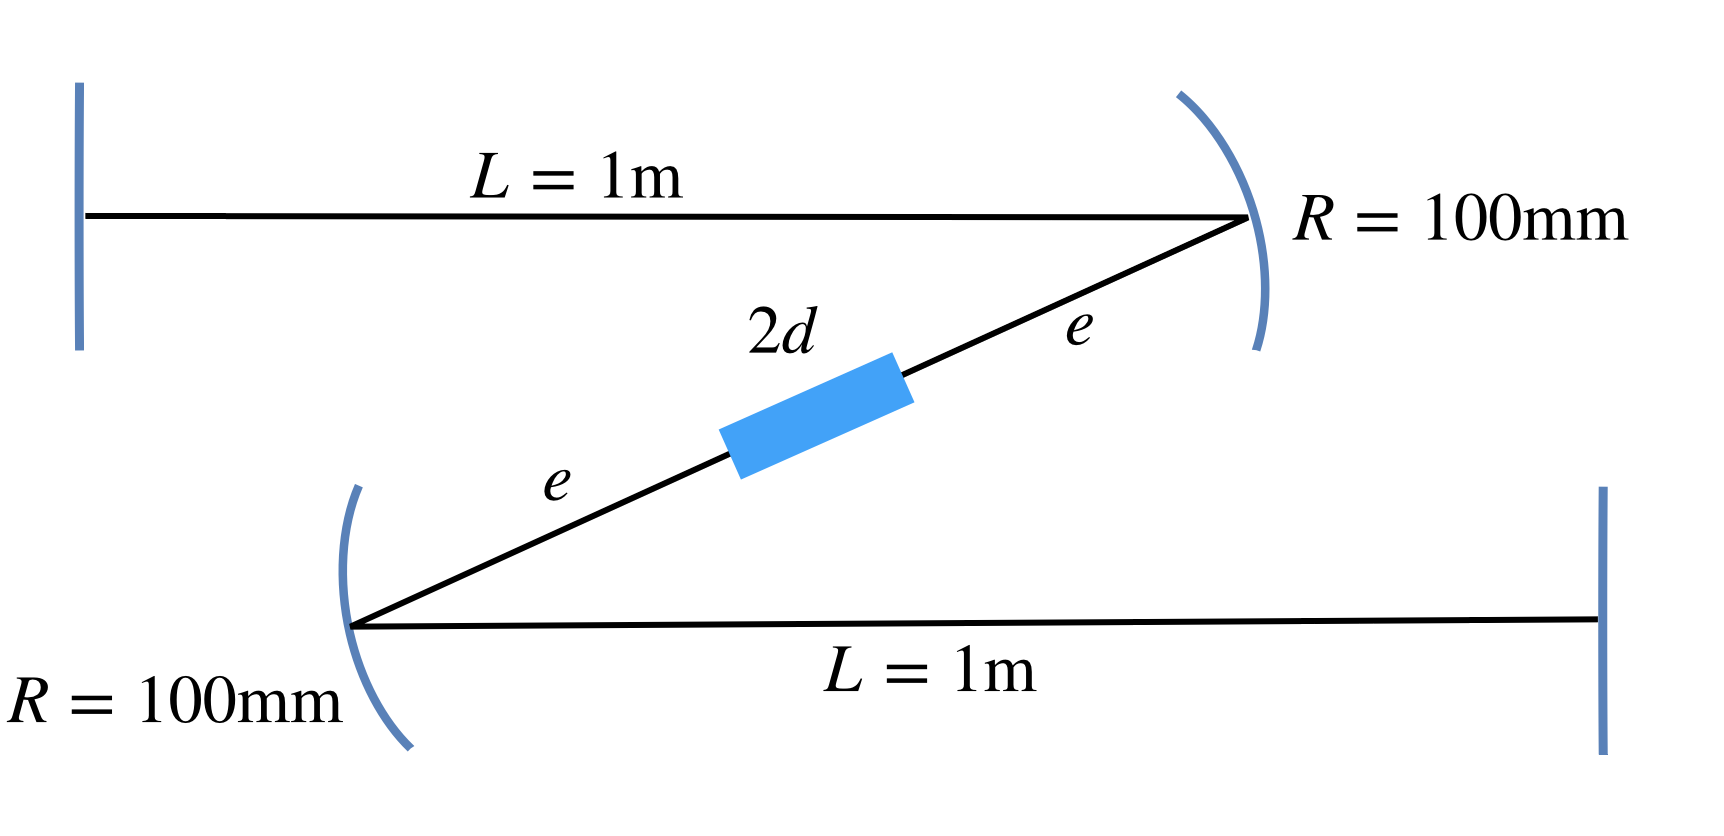
\includegraphics[width=7cm]{pictures/ZCav.png}
\end{center}
\end{figure}

Trouvez une cavité équivalente de la forme suivante :


 
\begin{figure}[!htbp]
\begin{center}
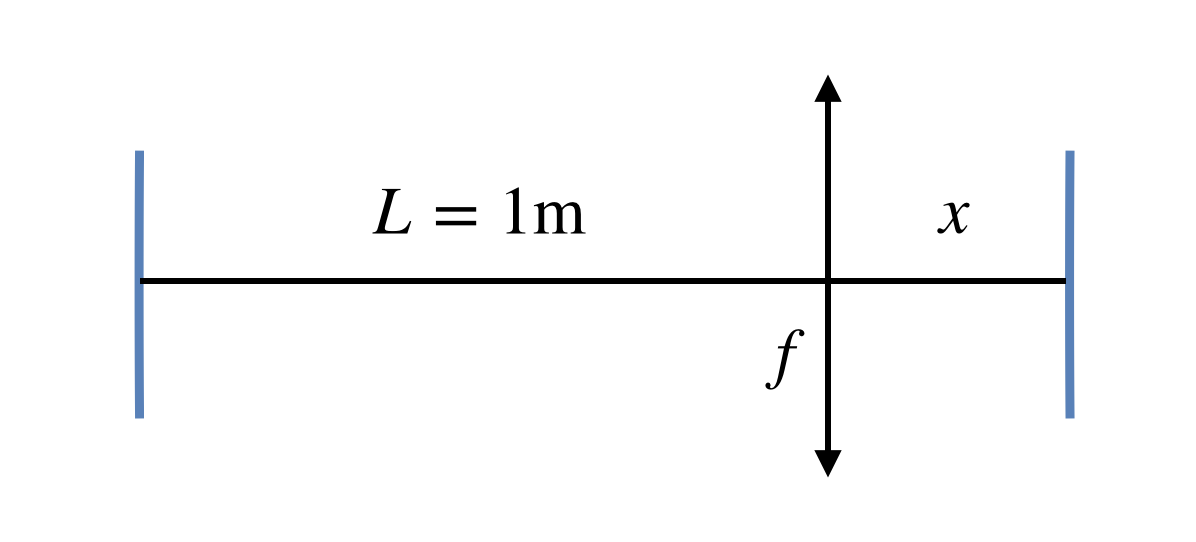
\includegraphics[width=5cm]{pictures/EqCav.png}
\end{center}
\end{figure}
Le rayon de courbure des miroirs est de 100$\,$mm. Calculer la matrice de transfert de la cavité. En déduire les conditions sur $x$ pour que la cavité soit stable.

Il existe une méthode plus simple pour trouver la zone de stabilité de la cavité. Elle consiste à utiliser le fait qu’un waist est positionné sur les miroirs plans. On définit $z$ et $z’$, les distances de $M_1$ et $M_2$ par rapport aux foyers $F$ et $F’$ de la lentille.
Trouver la relation entre $z$, $z’$ et $Z_R$.
Quand la cavité est stable, cette relation est vérifiée. En déduire la zone de stabilité ($x$ est la variable).
On se place au milieu de la zone de stabilité. Donner la valeur de $w_0$ et $w_0'$ sur les miroirs $M_1$ et $M_2$ (Application numérique $\lambda = 800\,$nm).

\end{exercice}


\end{document}
